\documentclass[a4paper,12pt]{article}
\usepackage{graphicx}
\usepackage{amsmath}
\usepackage{listings}
\usepackage{geometry}
\usepackage{hyperref}
\usepackage{color}
\usepackage{caption}
\usepackage{subcaption}
\usepackage{enumitem}
\usepackage{float}
\geometry{margin=1in}

\title{\textbf{Smart Home Automation and Security System with Human Detection}\\}
\author{Jerin Romijah Tuli \\ Roll: 2003056 \\ Section: A \\ Department of CSE \\ Rajshahi University Of Engineering And Technology}
\date{\today}

\begin{document}

\maketitle

\section{Introduction}
In this project, we develop an integrated home automation and security system utilizing an Arduino Uno microcontroller. The system enhances home security by first detecting human presence using an ultrasonic sensor. Upon detection, it prompts the user to enter a password via a keypad to unlock the door. Once unlocked, the system transitions into an automation mode, controlling lighting based on ambient light and occupancy, while also monitoring gas levels for safety. A Liquid Crystal Display (LCD) provides real-time feedback to the user regarding the system's status and sensor readings.

\section{Components Used}
The system comprises the following components:
\begin{itemize}
    \item \textbf{Arduino Uno}: Central microcontroller managing inputs from sensors and keypad, and controlling outputs such as the door lock and relay modules.
    \item \textbf{Liquid Crystal Display (LCD)}: Displays user prompts, lock status, and sensor data.
    \item \textbf{4x4 Keypad}: Input device for entering the unlock password.
    \item \textbf{Ultrasonic Sensor (HC-SR04)}: Detects human presence by measuring distance.
    \item \textbf{PIR Sensor}: Detects motion to determine occupancy for home automation.
    \item \textbf{Gas Sensor (MQ-2)}: Monitors gas levels to detect potential leaks.
    \item \textbf{Light Dependent Resistor (LDR)}: Measures ambient light levels to control lighting.
    \item \textbf{Relay Module}: Controls external electrical devices like lights based on sensor inputs.
    \item \textbf{EEPROM}: Stores the master password securely for the lock mechanism.
\end{itemize}

\section{System Design}
The system is architected to prioritize security by incorporating human detection before granting access through a password mechanism. Upon successful authentication, it seamlessly transitions into an automation mode to manage home utilities efficiently.

\subsection{Circuit Overview}
The Arduino Uno serves as the core of the system, interfacing with various sensors and output modules. The ultrasonic sensor is connected to digital pins 6 and 7 for triggering and echo, respectively. The LCD is interfaced using digital pins 2, 3, 4, 5, 11, and 12. The keypad is connected to analog pins A2 to A5 and digital pins 0, 1, 9, and 10. Sensors like PIR, LDR, and gas sensor are connected to designated analog and digital pins, while the relay module controls the lighting system based on sensor inputs.

\begin{figure}[H]
  \centering
  \begin{subfigure}{0.45\textwidth}
      \centering
      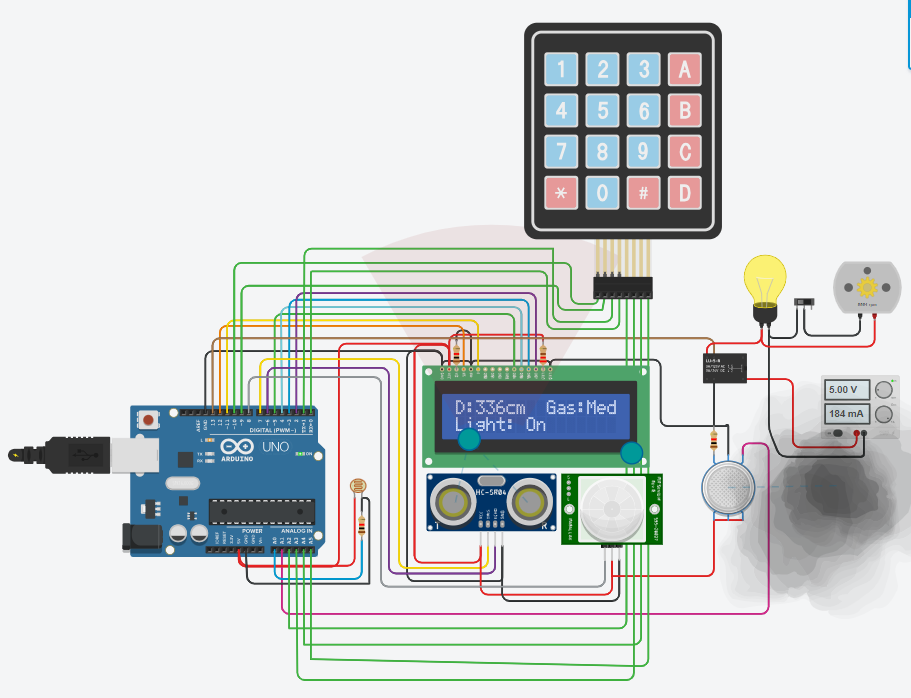
\includegraphics[width=\linewidth]{ultimate.png}
      \caption{Circuit design (circuit view)}
  \end{subfigure}
  \hfill
  \begin{subfigure}{0.45\textwidth}
      \centering
      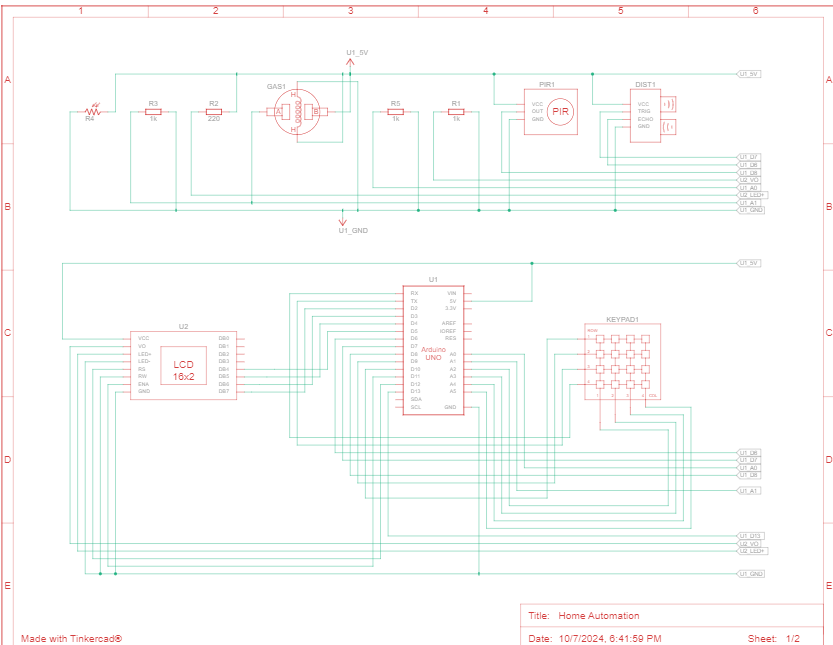
\includegraphics[width=\linewidth]{co_1.png}
      \caption{Circuit design (Schematic view)}
  \end{subfigure}
  \caption{Circuit Diagram of the Smart Home Automation and Security System with Human Detection}
  \label{fig:home_automation_circuit}
\end{figure}

\subsection{Operation}
\begin{enumerate}
    \item \textbf{Human Detection}: The ultrasonic sensor continuously measures the distance to detect human presence within a predefined threshold (e.g., 20 cm). If a human is detected, the system prompts the user to enter a password.
    
    \item \textbf{Password Entry}: Upon human detection, the LCD displays a password entry prompt. The user inputs the password via the keypad. The system verifies the entered password against the stored master password in the EEPROM.
    
    \item \textbf{Authentication}:
    \begin{itemize}
        \item \textbf{Correct Password}: The door unlocks, and the system enters automation mode, controlling home utilities based on sensor data.
        \item \textbf{Incorrect Password}: An error message is displayed, and the system prompts for password entry again.
    \end{itemize}
   
    \item \textbf{Home Automation}: In automation mode, the system manages lighting based on ambient light detected by the LDR and occupancy detected by the PIR sensor. It also monitors gas levels using the gas sensor, triggering alerts if dangerous levels are detected.
\end{enumerate}

\section{Code Implementation}
The following Arduino code governs the operation of the home automation and security system. It integrates human detection, password authentication, and automation features, ensuring a secure and efficient smart home environment.

% Define custom colors for code
\definecolor{commentColor}{rgb}{0.12, 0.38, 0.18}
\definecolor{keywordColor}{rgb}{0.25, 0.36, 0.79}
\definecolor{stringColor}{rgb}{0.64, 0.08, 0.08}
\definecolor{backcolour}{rgb}{0.95,0.95,0.92}

\lstset{
    backgroundcolor=\color{backcolour}, 
    language=C++,                    % Set language
    basicstyle=\ttfamily\footnotesize,% Code font
    keywordstyle=\color{keywordColor}\bfseries, % Keywords in blue
    commentstyle=\color{commentColor}\itshape,  % Comments in green and italic
    stringstyle=\color{stringColor},  % Strings in red
    numbers=left,                     % Line numbers on the left
    numberstyle=\tiny,                % Line number font size
    stepnumber=1,                     % Step between two line numbers
    breaklines=true,                  % Automatic line breaking
    frame=single,                     % Single frame around the code
    captionpos=b,                     % Caption position at the bottom
    showstringspaces=false            % Don't show spaces in strings
}

\begin{lstlisting}[language=C++, caption={Arduino Code for Smart Home Automation and Security System}]
#include <LiquidCrystal.h>
#include <Keypad.h>
#include <EEPROM.h>

// LCD and Keypad for door lock
#define Password_Length 5
const int rs = 12, en = 11, d4 = 5, d5 = 4, d6 = 3, d7 = 2;
LiquidCrystal lcd(rs, en, d4, d5, d6, d7);

const byte ROWS = 4;
const byte COLS = 4;
char keys[ROWS][COLS] = {
  {'1', '2', '3', 'A'},
  {'4', '5', '6', 'B'},
  {'7', '8', '9', 'C'},
  {'*', '0', '#', 'D'}
};
byte rowPins[ROWS] = {10, 9, 1, 0};
byte colPins[COLS] = {A2, A3, A4, A5};
Keypad keypad = Keypad(makeKeymap(keys), rowPins, colPins, ROWS, COLS);

char Data[Password_Length];
char Master[Password_Length];
byte data_count = 0;
char key;
byte mode = 0;  // 0 for locked, 1 for unlocked

// Sensor and relay pins for home automation
int releNO = 13;
int inputPir = 8;
int sensorLDR = A0;
int PINO_SGAS = A1;
int distanceThreshold = 20;  // Threshold set to 20 cm
int cm = 0;
long readUltrasonicDistance(int triggerPin, int echoPin);

// Variables to store previous sensor values
int previousCm = -1;
int previousGasLevel = -1;

// Variable to track human detection
bool humanDetected = false;
bool enterPasswordDisplayed = false;  // New flag to control LCD updates for password

// Function for checking password
void Check_EEPROM() {
  EEPROM.get(0, Master);
  if (Master[0] == 0 && Master[1] == 0 && Master[2] == 0 && Master[3] == 0) {
    char FirstTimePassword[] = {'1', '2', '3', '4'};
    EEPROM.put(0, FirstTimePassword);
    EEPROM.get(0, Master);
  }
}

void setup() {
  Serial.begin(9600);
  lcd.begin(16, 2);
  pinMode(releNO, OUTPUT);
  pinMode(inputPir, INPUT);
  pinMode(sensorLDR, INPUT);
  Check_EEPROM();
}

void loop() {
  // Read distance from ultrasonic sensor
  cm = 0.01723 * readUltrasonicDistance(7, 6);

  // Human detected within threshold distance
  if (!humanDetected && cm <= distanceThreshold) {
    lcd.clear();
    lcd.setCursor(0, 0);
    lcd.print("Human detected!");
    delay(1000);  // Wait for 1 second
    humanDetected = true;  // Mark human as detected
    lcd.clear();
    enterPasswordDisplayed = false;  // Reset flag for password prompt
  }

  if (humanDetected && mode == 0) {  // Prompt for password after detection
    if (!enterPasswordDisplayed) {
      lcd.clear();
      lcd.setCursor(0, 0);
      lcd.print("Enter Password:");
      enterPasswordDisplayed = true;  // Ensure password prompt is displayed only once
    }

    key = keypad.getKey();
    if (key) {
      Data[data_count] = key;
      lcd.setCursor(4 + data_count, 1);
      lcd.print("*");
      data_count++;
    }

    if (data_count == Password_Length - 1) {
      if (!strcmp(Data, Master)) {  // Password correct
        lcd.clear();
        lcd.setCursor(0, 0);
        lcd.print("Unlocking...");
        delay(2000);
        lcd.clear();
        lcd.setCursor(0, 0);
        lcd.print("Door Unlocked");
        mode = 1;  // Switch to home automation
        humanDetected = false;  // Reset human detection after unlocking
        delay(2000);
        lcd.clear();
        enterPasswordDisplayed = false;  // Reset flag
      } else {  // Incorrect password
        lcd.clear();
        lcd.setCursor(0, 0);
        lcd.print("Incorrect Pass");
        delay(2000);
        lcd.clear();
        lcd.setCursor(0, 0);
        lcd.print("Enter Password:");  // Re-display password prompt
        enterPasswordDisplayed = true;  // Keep password prompt displayed
      }
      data_count = 0;  // Reset password input
    }
  }

  // Home automation activates only after the door is unlocked
  if (mode == 1) {
    int val = digitalRead(inputPir);
    int resuldoSensorLDR = analogRead(sensorLDR);
    int gasLevel = analogRead(PINO_SGAS);

    // Update LCD for distance reading
    if (cm != previousCm) {
      lcd.setCursor(0, 0);
      lcd.print("D:");
      lcd.print(cm);
      lcd.print("cm  ");
      previousCm = cm;  // Store the current distance
    }

    // LDR and PIR control
    if (resuldoSensorLDR < 600 && val == HIGH) {
      digitalWrite(releNO, HIGH);
      lcd.setCursor(0, 1);
      lcd.print("Light: On ");
      delay(5000);
    } else {
      digitalWrite(releNO, LOW);
      lcd.setCursor(0, 1);
      lcd.print("Light: Off");
      delay(300);
    }

    // Update LCD for gas sensor reading
    if (gasLevel != previousGasLevel) {
      lcd.setCursor(8, 0);
      lcd.print(" Gas:");  
      if (gasLevel <= 85) {
        lcd.print("Low  ");  
      } else if (gasLevel <= 120) {
        lcd.print("Med  ");
      } else if (gasLevel <= 200) {
        lcd.print("High ");
      } else if (gasLevel <= 300) {
        lcd.print("Ext  ");
      }
      previousGasLevel = gasLevel;  // Store the current gas level
    }

    delay(250);  // Add delay for smooth display
  }
}

// Ultrasonic sensor function
long readUltrasonicDistance(int triggerPin, int echoPin) {
  pinMode(triggerPin, OUTPUT);
  digitalWrite(triggerPin, LOW);
  delayMicroseconds(2);
  digitalWrite(triggerPin, HIGH);
  delayMicroseconds(10);
  digitalWrite(triggerPin, LOW);
  pinMode(echoPin, INPUT);
  return pulseIn(echoPin, HIGH);
}
\end{lstlisting}

\section{Results and Discussion}
The implemented system successfully integrates human detection with a secure password mechanism, followed by home automation functionalities. The ultrasonic sensor reliably detects human presence within the set threshold, prompting the LCD to request password entry. Upon entering the correct password, the system unlocks the door and transitions into automation mode. The LCD provides clear feedback throughout the process, enhancing user interaction.

In automation mode, the LDR and PIR sensor effectively control the lighting based on ambient light and occupancy, ensuring energy efficiency. The gas sensor accurately monitors gas levels, displaying appropriate warnings and ensuring safety by alerting users in case of hazardous gas concentrations. The use of EEPROM ensures that the master password is stored securely, preventing unauthorized access.

% Modifications for figure numbering
\makeatletter
\renewcommand{\thesubfigure}{\@alph\c@subfigure} % Use lowercase alphabet for subfigure numbering
\setcounter{subfigure}{0} % Start subfigure numbering from 'g'

\begin{figure}[H]
  \centering
  \begin{subfigure}{0.45\textwidth}
      \centering
      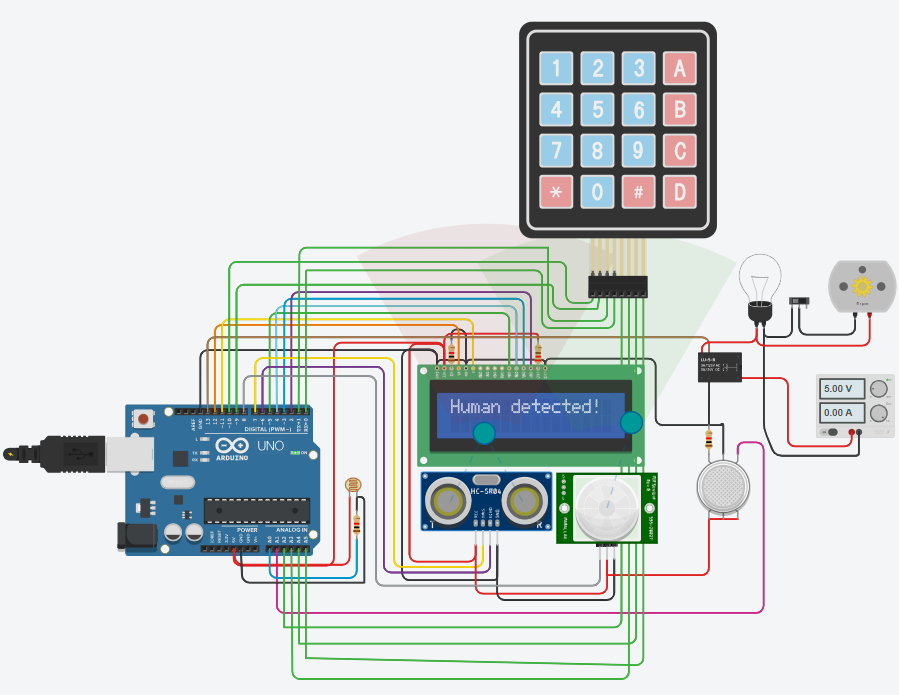
\includegraphics[width=\linewidth]{circuit_overview4.png}
      \caption{Ultrasonic sensor continuously detects human presence and triggered password prompt}
  \end{subfigure}
  \hfill
  \begin{subfigure}{0.45\textwidth}
      \centering
      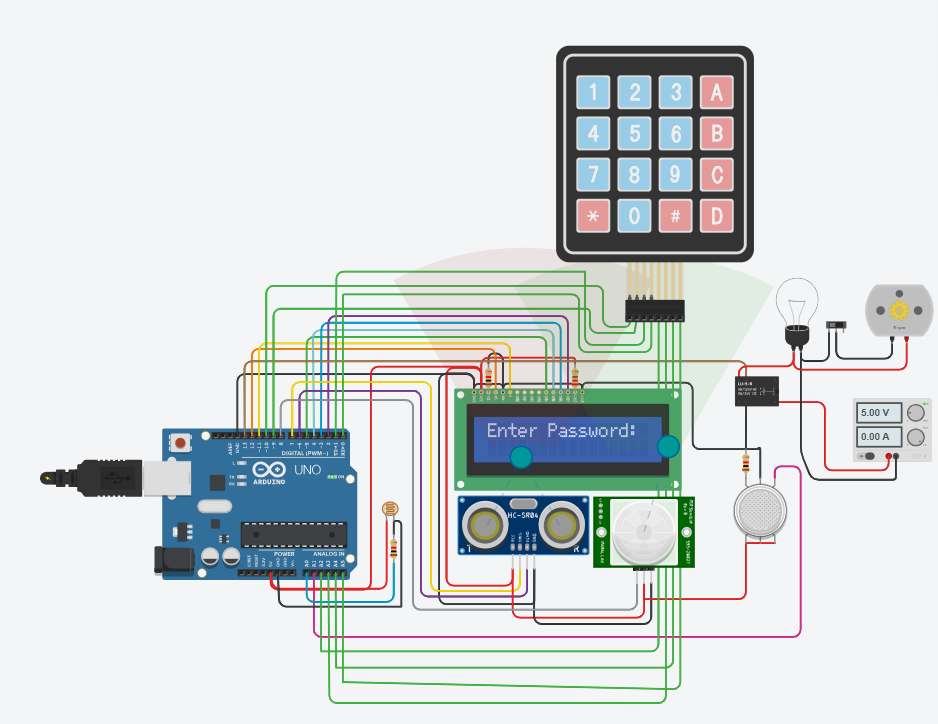
\includegraphics[width=\linewidth]{circuit_overview2.png}
      \caption{House holder will give 4 digit password to unlock the door}
  \end{subfigure}
  
  \vspace{1em} % Adds space between rows of images

  \begin{subfigure}{0.45\textwidth}
      \centering
      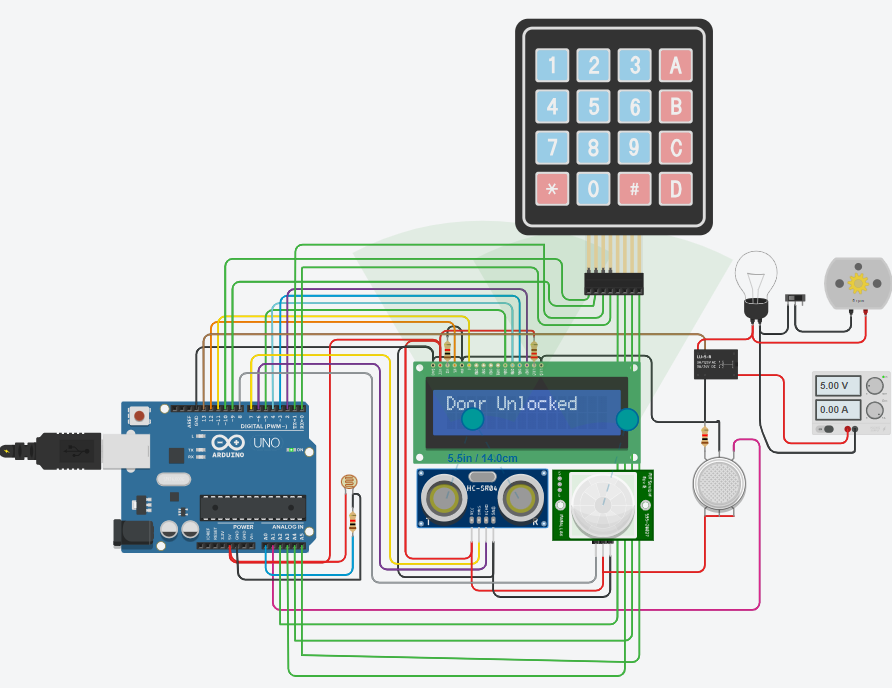
\includegraphics[width=\linewidth]{circuit_overview1.png}
      \caption{Door Unlocked!}
  \end{subfigure}
  \hfill
  \begin{subfigure}{0.45\textwidth}
      \centering
      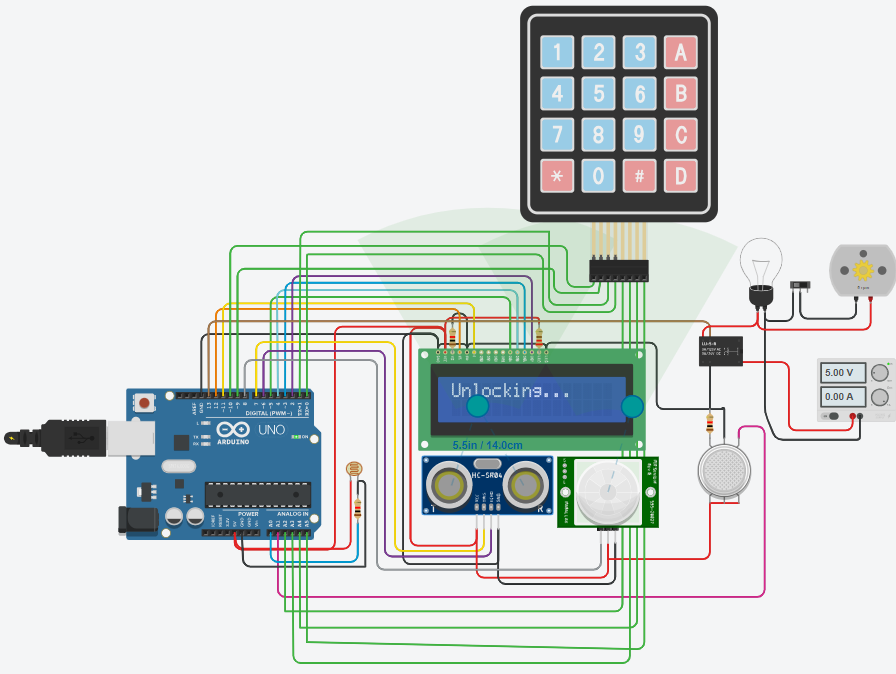
\includegraphics[width=\linewidth]{circuit_overview3.png}
      \caption{Unlocking}
  \end{subfigure}
  
  \vspace{1em} 
  \begin{subfigure}{0.45\textwidth}
    \centering
    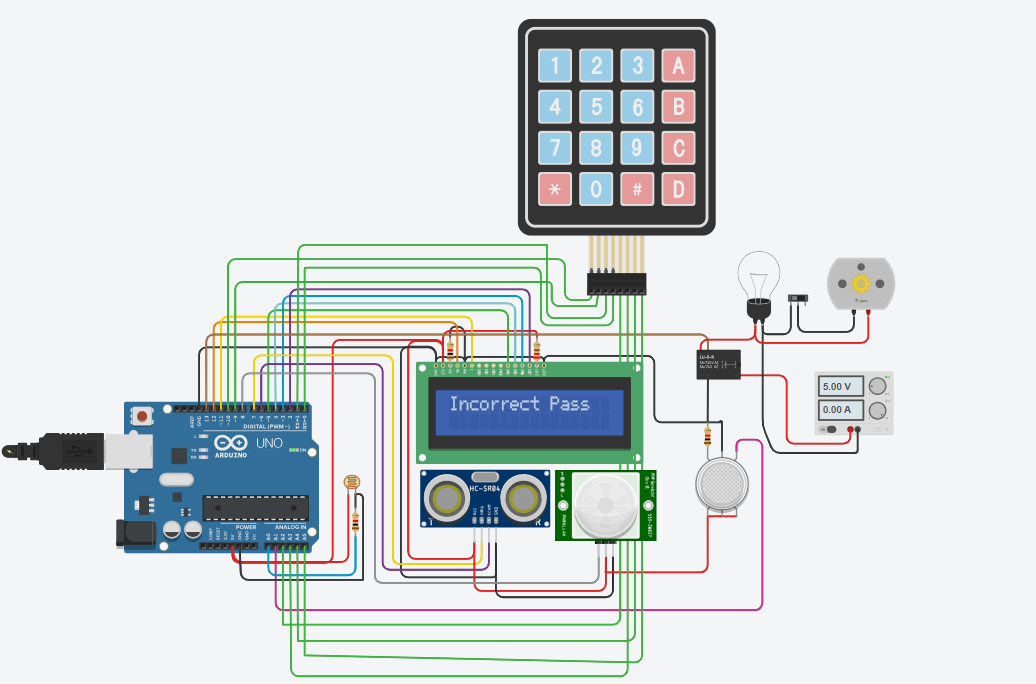
\includegraphics[width=\linewidth]{incorrect.png}
    \caption{The entered password is incorrect.}
  \end{subfigure}
  \hfill
  \begin{subfigure}{0.45\textwidth}
      \centering
      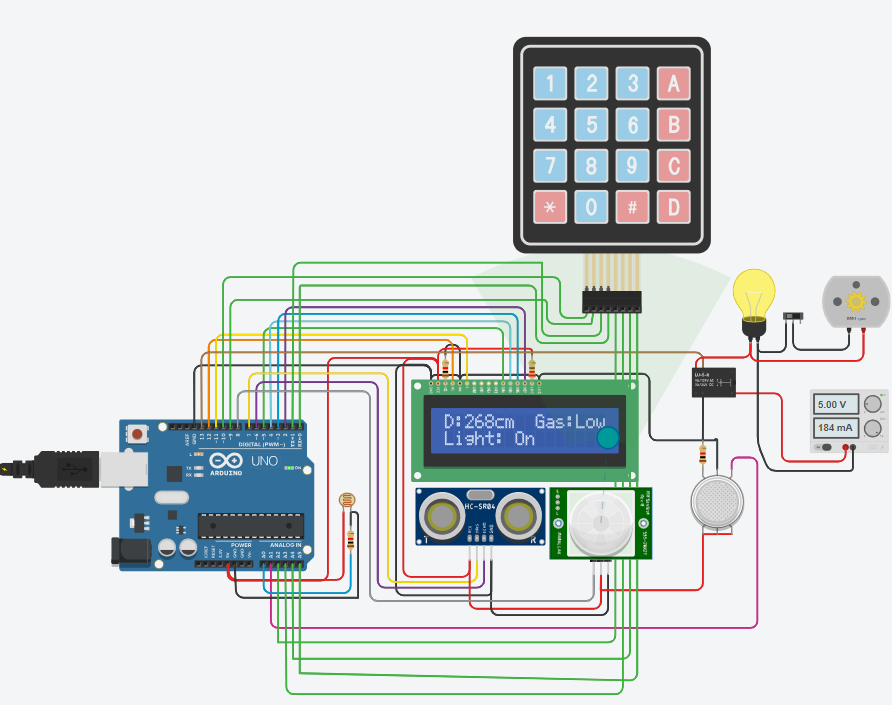
\includegraphics[width=\linewidth]{pirsensor1.png}
      \caption{Pir sensor detects human presence and switches on the light and DC fan; a Relay module acts as an external switch.}
  \end{subfigure}
  \caption{Operational feedback from the Smart Home Automation and Security System}
  \label{fig:operational_feedback}
\end{figure}

\begin{figure}[H]
  \centering
  \begin{subfigure}{0.45\textwidth}
      \centering
      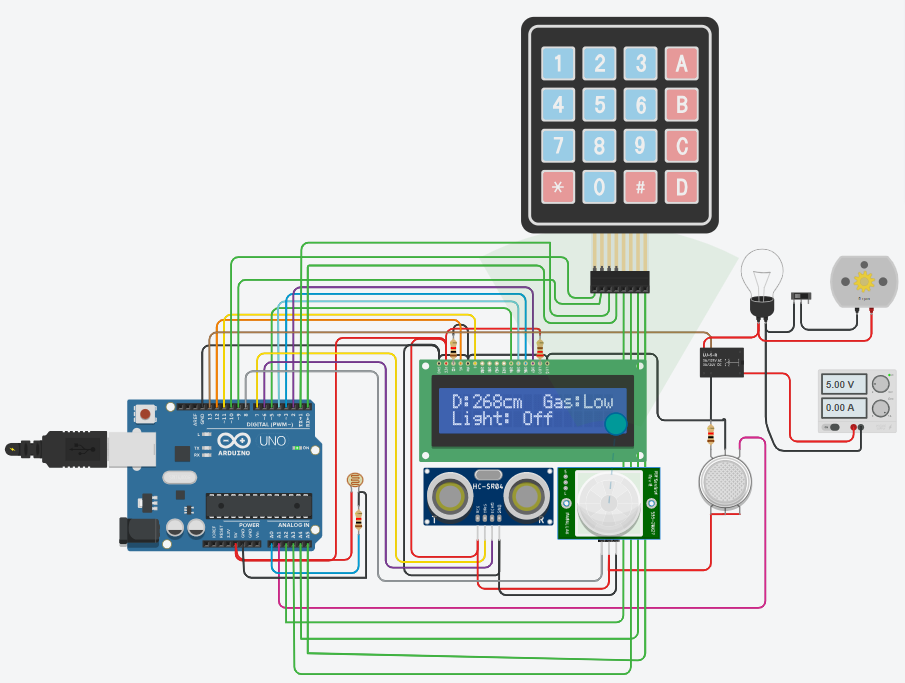
\includegraphics[width=\linewidth]{gassensor1.png}
      \caption{Gas sensor detects the gas level continuously.}
  \end{subfigure}
  \hfill
  \begin{subfigure}{0.45\textwidth}
      \centering
      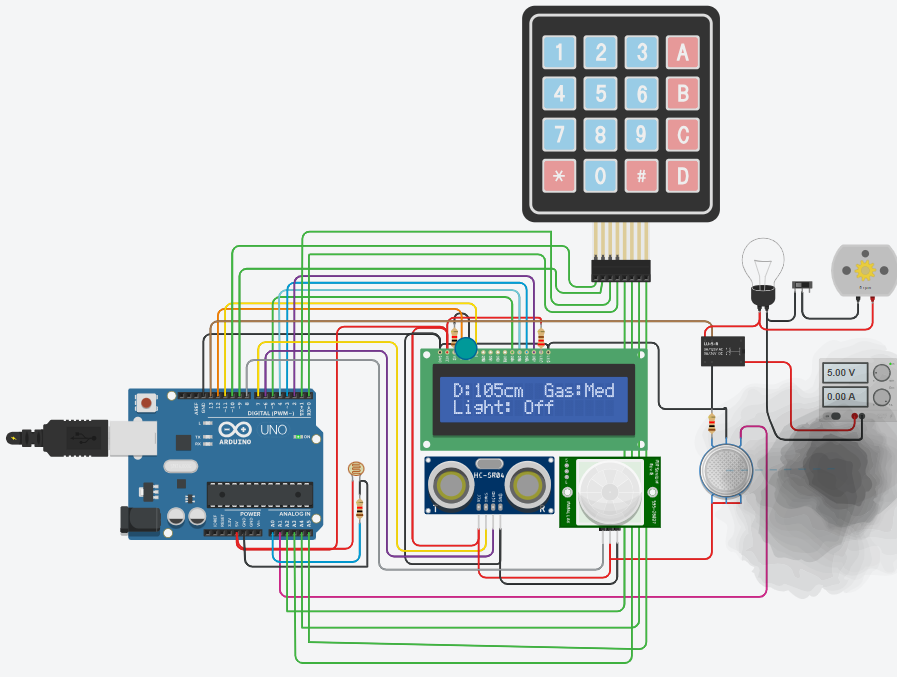
\includegraphics[width=\linewidth]{gassensor3.png}
      \caption{Gas sensor detects the gas level and alerts the user. If there is medium level gas leakage, it shows "Med".}
  \end{subfigure}

  \vspace{1em}

  \begin{subfigure}{0.45\textwidth}
      \centering
      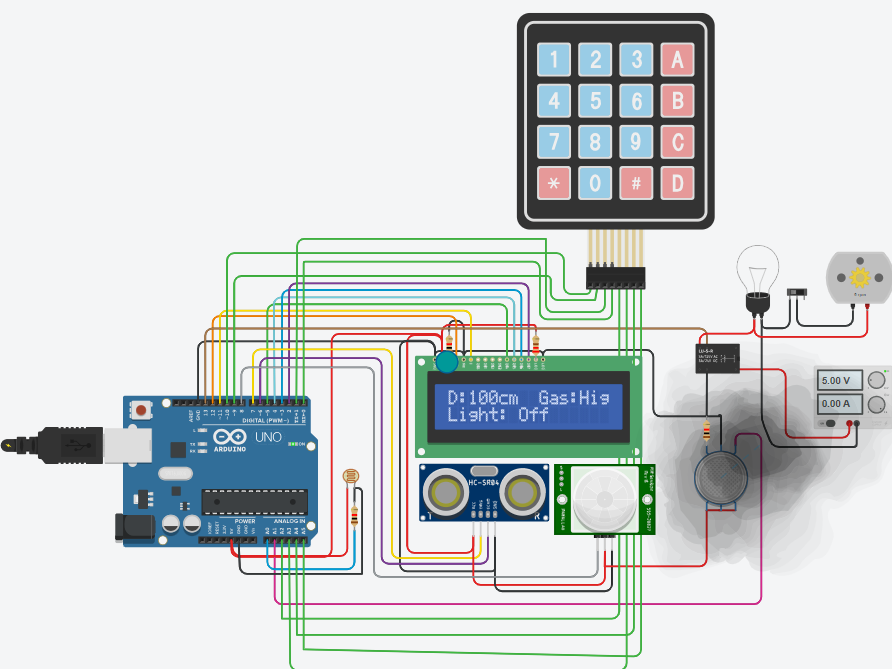
\includegraphics[width=\linewidth]{gassensor4.png}
      \caption{If there is high level gas leakage, it shows "High".}
  \end{subfigure}
  \hfill
  \begin{subfigure}{0.45\textwidth}
      \centering
      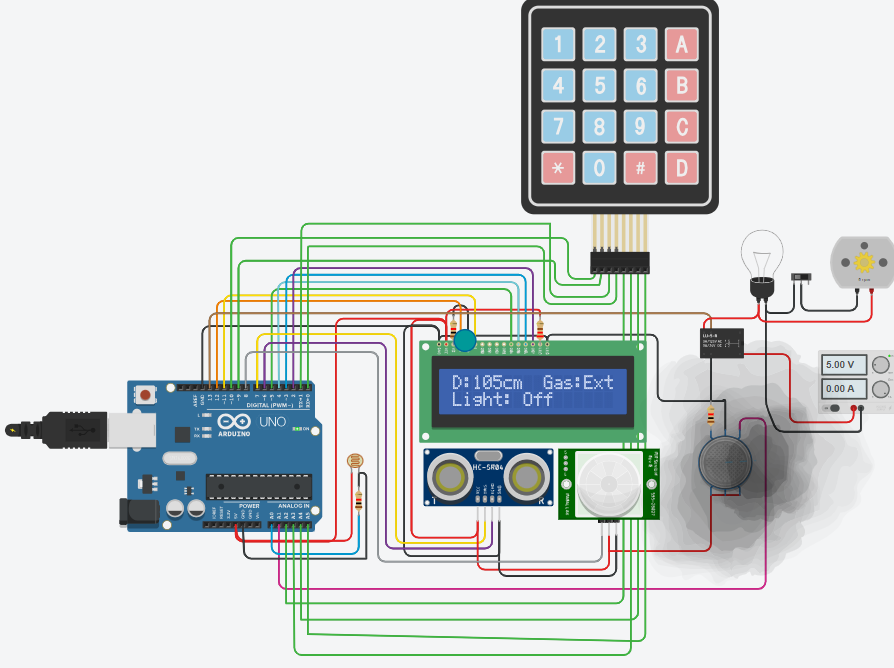
\includegraphics[width=\linewidth]{gassensor2.png}
      \caption{If the gas level is higher than the threshold, it shows "Exit".}
  \end{subfigure} 

  \caption{Operational feedback from the  Gas Sensor .}
  \label{fig:circuit_overview}
\end{figure}

\section{Conclusion}
This project demonstrates the effective integration of security and automation in a smart home system using Arduino. By prioritizing human detection before authentication, the system enhances security measures. The seamless transition to home automation post-authentication optimizes energy usage and ensures environmental safety. Future enhancements could include wireless connectivity for remote monitoring, integration with mobile applications, and expanding the range of controlled devices for a more comprehensive smart home experience.

\section{References}
\begin{thebibliography}{9}

\bibitem{ArduinoUno}
Arduino Uno, \emph{Arduino Documentation}. Available at: \url{https://www.arduino.cc/en/Guide/ArduinoUno}.

\bibitem{LiquidCrystal}
LiquidCrystal Library, \emph{Arduino Documentation}. Available at: \url{https://www.arduino.cc/en/Reference/LiquidCrystal}.

\bibitem{Keypad}
Keypad Library, \emph{Arduino Playground}. Available at: \url{https://playground.arduino.cc/Code/Keypad/}.

\bibitem{PIRSensor}
PIR Sensor, \emph{SparkFun Guide}. Available at: \url{https://www.sparkfun.com/products/13285}.

\bibitem{LDR}
LDR Working, \emph{Electronics Tutorials}. Available at: \url{https://www.electronics-tutorials.ws/io/ldr.html}.

\bibitem{GasSensor}
Gas Sensor (MQ-2), \emph{Datasheet}. Available at: \url{https://www.sparkfun.com/datasheets/Sensors/Biometric/MQ-2.pdf}.

\bibitem{EEPROM}
EEPROM Library, \emph{Arduino Documentation}. Available at: \url{https://www.arduino.cc/en/Reference/EEPROM}.

\bibitem{Ultrasonic}
Ultrasonic Sensor HC-SR04, \emph{SparkFun Guide}. Available at: \url{https://www.sparkfun.com/products/15569}.

\bibitem{Relay}
Relay with Arduino, \emph{Last Minute Engineers Tutorial}. Available at: \url{https://lastminuteengineers.com/arduino-relay-tutorial/}.

\end{thebibliography}

\end{document}